\chapter{実装}
\section{概要}
\SysName は、ハードウェアとして三角法を用いた光学式距離センサ10個を一列に並べたセンサアレイと、センサから取得した値の処理と値を元に座標を計算するソフトウェアからなる。
\section{プロトタイプ1} 
\secLabel{proto1}
\subsection{ハードウェア}
距離センサはSHARP GP2Y0E03\footnote{http://www.sharp.co.jp/products/device/lineup/selection/opto/haca/diagram2.html}を使用した。この距離センサは三角測量の原理を用い、対象までの距離を計測する。本センサの値の取得には、Arduino MEGA 2560を用いる。距離センサとは\iic を用いて接続を行う。個々のセンサは、スレーブアドレスが初期値(0x40)で統一されているために、アプリケーションノート\footnote{http://www.sharp.co.jp/products/device/doc/opto/gp2y0e02\_03\_appl\_j.pdf}に記載されているe-fuseプログラミングの手順で、スレーブアドレスの変更を行なっている。これにより、10個の距離センサを2本の信号線で制御する。
接続した距離センサは1列に並べる。\SysName では、長さ約30\si{cm}のプラスティック製の定規を用意し、両面テープでセンサ本体を固定し、配線類をセロハンテープで固定した。装置が長細いため、接続にはブレッドボードの電源とグランド接続に用いられる部分を2列使用した。\refImg{ig1}は実際に製作したプロトタイプの1つである。\refImg{ig1}ではセンサごとの間隔は約11\si{mm}としている。
\begin{figure}[htbp]
	\begin{center}
		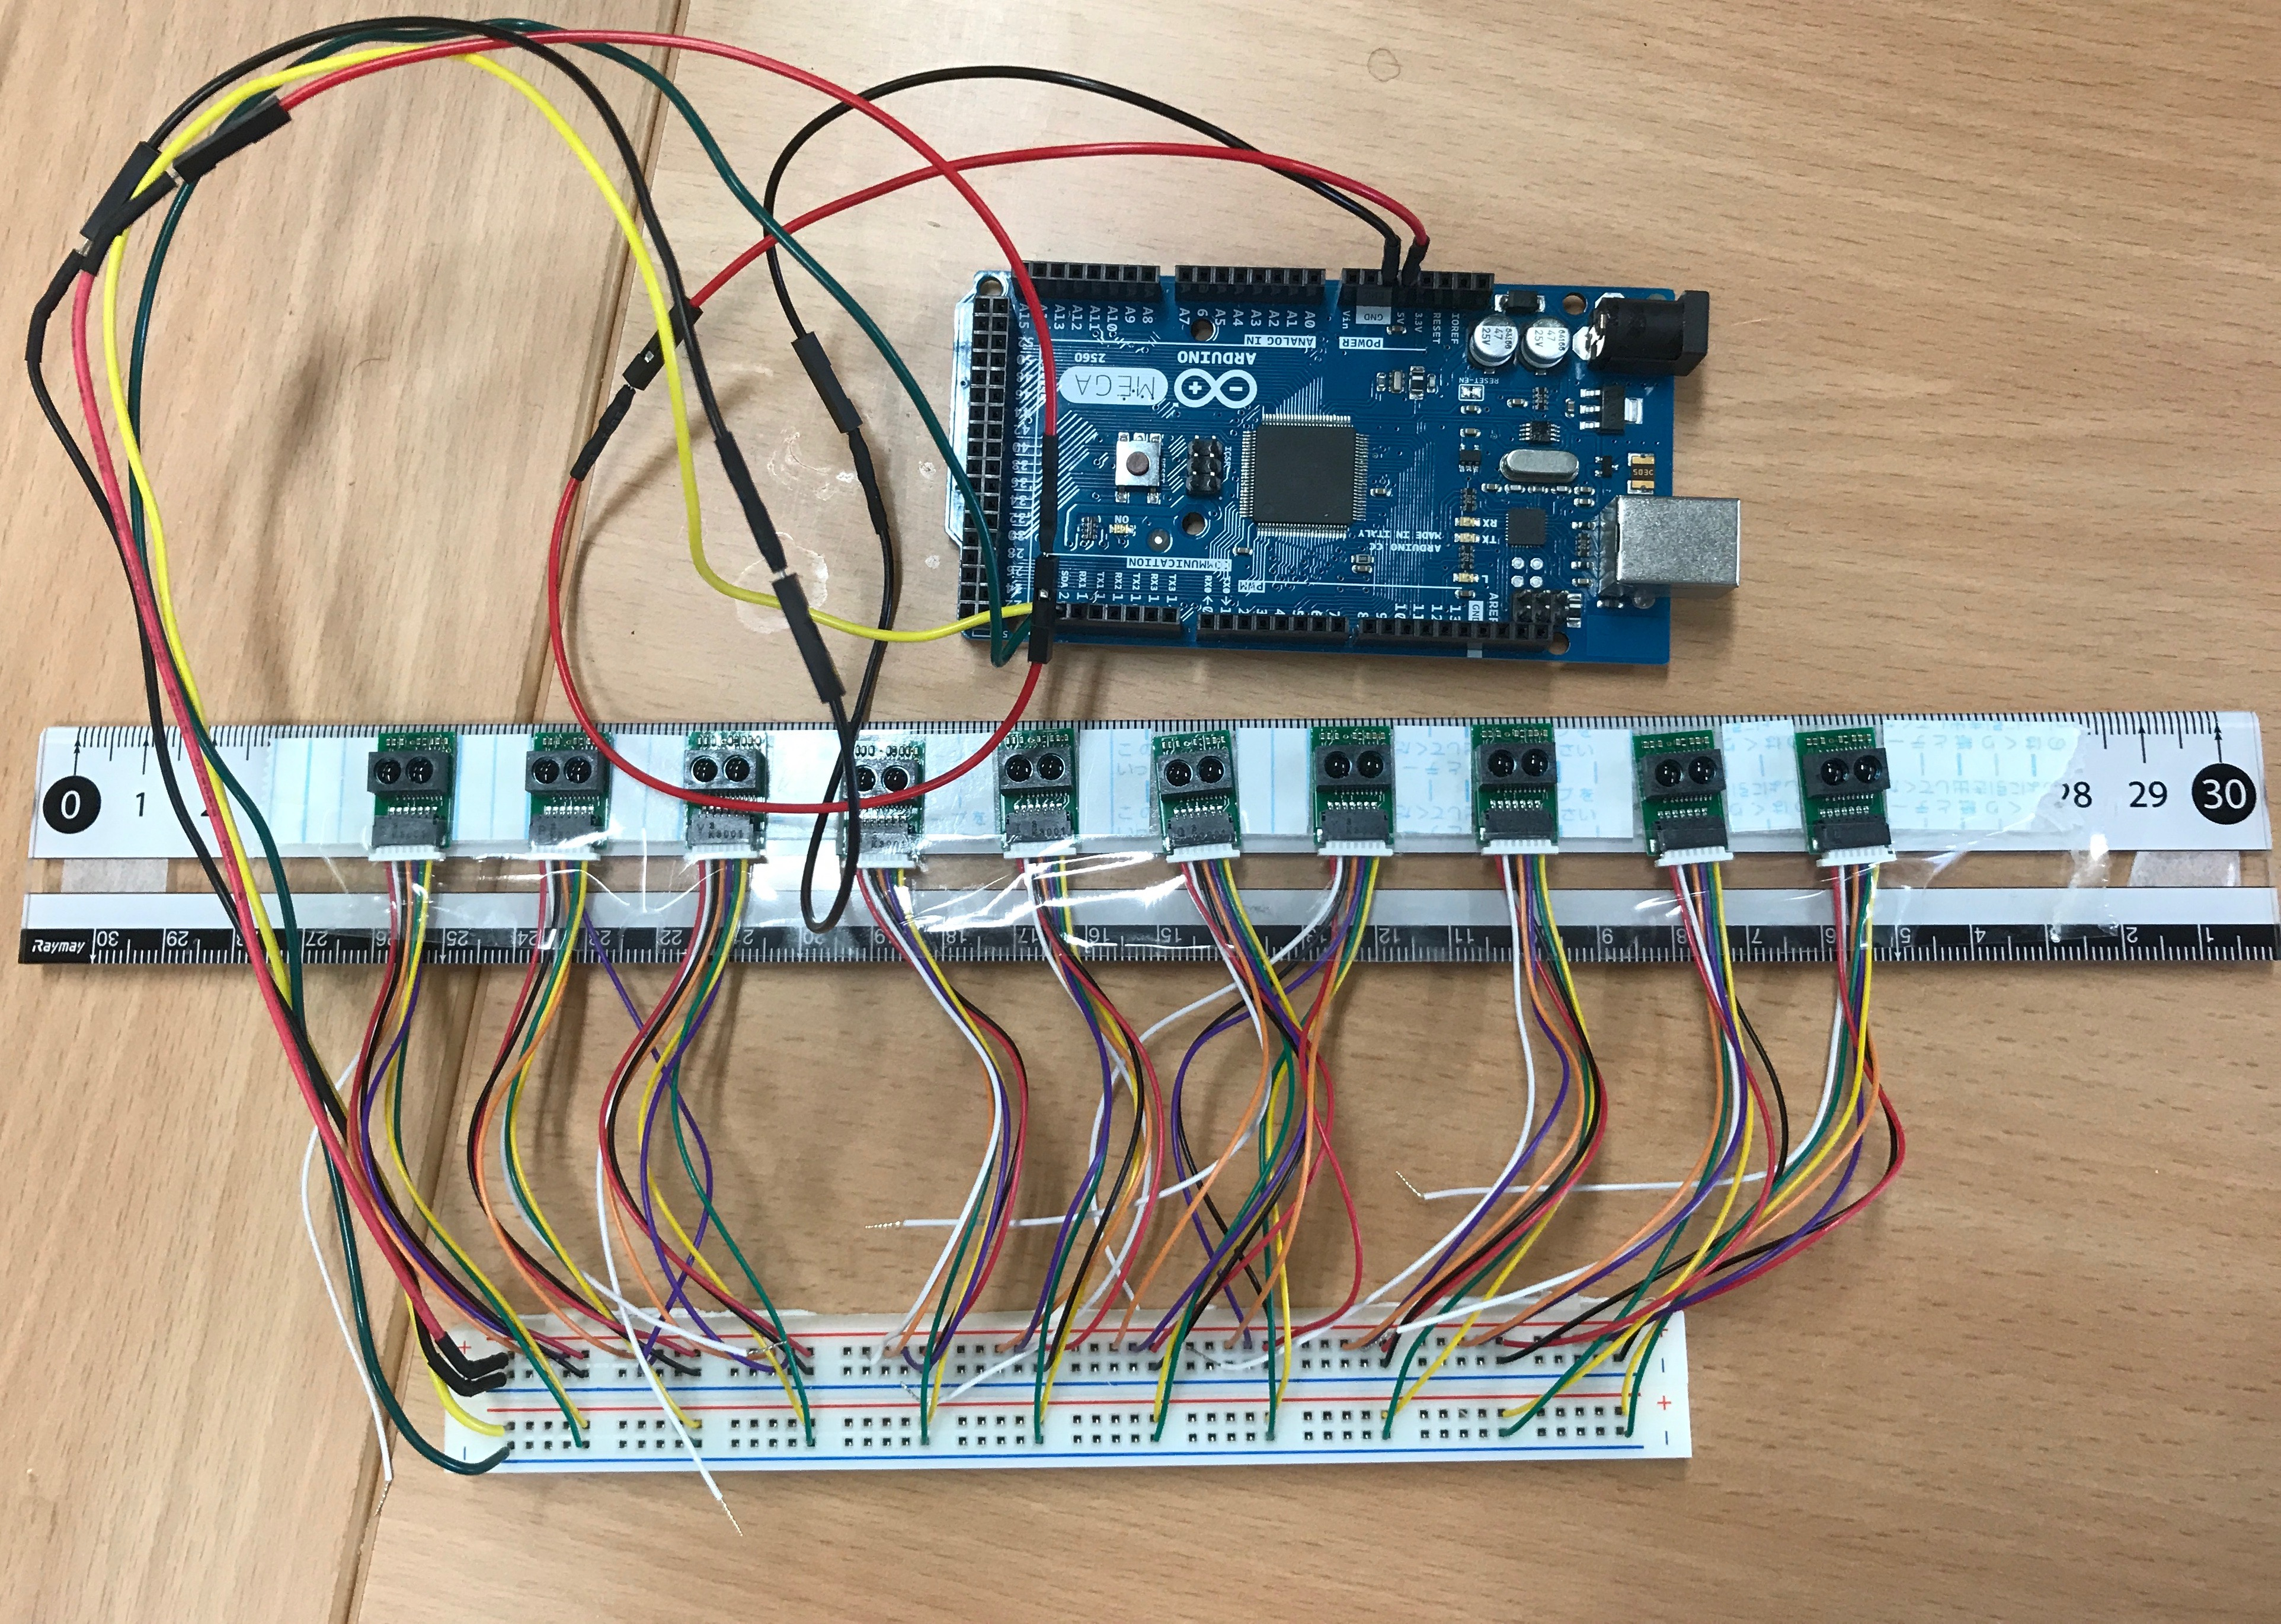
\includegraphics[width = 90mm]{./img/IMG_1794.jpg}
	\end{center}
	\caption{\fixme{プロトタイプその1}}
	\label{img:ig1}
\end{figure}
Arduinoでは、\iic による制御を行い、値をシリアルモニタに送信することだけを行う。したがって、センサのノイズ等の処理は全てソフトウェアで行う。
\subsection{ソフトウェア} 
プログラム言語はPythonを用いた。シリアル通信のためのライブラリとしてPySerial、ポインタを描画するGUIのためのライブラリとしてPyQtを用いた。
膝の位置の計算には、スマートウォッチに搭載した距離センサから指の位置をトラッキングしたXiaoら\cite{Xiao:2018:LOP:3173574.3173669}の研究を参考にした。膝の位置の計算は次のように行う。
\begin{enumerate}
	\item センサからの値を指数平均平滑フィルタを用いて平滑化する。
	\item $y$軸方向の位置をすべての距離センサの最小値とする。
		\begin{eqnarray}
		 	y = min(sensors\_val)
		 	\label{formula:f1}
		\end{eqnarray}
	\item $i$番目の距離センサについて、重み$w_i$を式\ref{formula:f2}のように計算する。ここで、$d$は重み調整の定数である。\SysName では調整の結果$d=2$としている。
		\begin{eqnarray}
			w_i = \cfrac{1}{y_i - y + d}
		\label{formula:f2}
	\end{eqnarray}
	\item $w_i$から、$x$座標を式\ref{formula:f3}のように計算する。
		\begin{eqnarray}
		 	x =\cfrac{\sum iw_i}{\sum w_i}
		 	\label{formula:f3}
		\end{eqnarray} 
	\item ($x,y$)を指数平均平滑フィルタを用いて平滑化する。
	\item ($x,y$)を実際のディスプレイの画面サイズに合わせてマッピングする。
\end{enumerate}
使用者はあらかじめ上下左右方向にキャリブレーションを行い、膝の可動範囲の限界を記録し、これを元に6.のマッピングが行われる。

\subsection{プロトタイプ1の問題点}\subsecLabel{proto1_problem}
実装を行なったプロトタイプを机の裏に設置し、自由なポインタの操作ができるか試みた。キャリブレーション次第では膝を静止させた時にポインタも静止するが、多くの場合は膝を静止させているにも関わらずポインタは左右に振れるなどした。センサからの値を観察したところ、\fixme{膝がかかっていない部分の値}が激しく上下していることがわかった。原因として、以下のようなものが挙げられた。
\begin{enumerate}
	\item アプリケーションノートに、移動物体に対する正しいセンサの設置方向に関する記述があり、センサの設置方向が正しくない可能性がある。
	\item センサのコネクタのピンが細いため、ブレッドボード接続をしたことにより接触不良を起こしている。
	\item 床の色が黒く、赤外線を吸収し正しく距離を計測できていない。
	\item \fixme{センサの設置部分が小さく、膝が範囲外に飛び出してしまう}
\end{enumerate}
\section{プロトタイプ2}
\refSubsec{proto1_problem}であげた問題を解決するために、プロトタイプに改良を行った。1.について、すべてのセンサを90度左回転させて設置した。また同時に4.について、左右方向に膝を傾けた時にどれくらいの範囲を動くかを測定し、必要なセンサのカバー範囲を推定した。測定の結果、におよそ20〜30\si{cm}の長さが必要であるとわかった。このことから、センサの間隔を11\si{mm}から30\si{mm}に変更した。


